\documentclass[12pt,fleqn]{article}\usepackage{../common}
\begin{document}
Ders 2

Karakteristik Egriler Metodu

Bu metot katsayilari sabit olmayan 1. derece, lineer PDE cozmemize yardim
eder. PDE su formdadir

\[ \frac{\partial u}{\partial x} + 
p(x,y) \frac{\partial u}{\partial y} = 0 
\ \ \ (1)
 \]

ve $p(x,y)$, $x,y$ degiskenlerinin bir fonksiyonudur. 

Ustteki denklemi iki vektorun noktasal carpimi olarak ta gorebiliriz. 

\[ 
<\frac{\partial u}{\partial x}, \frac{\partial u}{\partial y}> \cdot 
<1,p(x,y)> = 0
 \]

Bu acidan bakinca yukaridaki ifade yeni bir sey soyluyor, $u$'nun
$<1,p(x,y)>$ vektorune gore yonsel turevinin sifir oldugunu soyluyor, yani
o yonde hicbir degisim yok. 

Simdi tek basina $<1,p(x,y)>$ vektorunu dusunelim, her degisik $x,y$ icin
bu vektorler bir vektor alani olusturur, bu alandaki vektorleri bir egrinin
``belli bir noktadaki egimini gosterdigi'' seklinde alabiliriz. O
noktalardaki egim $p(x,y) / 1$ olacaktir dogal olarak, o zaman bu egriler
icin soyle bir basit diferansiyel denklem (ODE) yazabiliriz.

\[ \frac{dy}{dx} = \frac{p(x,y)}{1} \]

ya da

\[ \frac{dy}{dx} = p(x,y) 
\ \ \ (2)
\]

Bu ODE bir yon alani (direction field) olusturur (bkz MIT OCW ODE Ders 1).

Simdi geri adim atip her seye tekrar bakalim. (1) diyor ki $x,y$ noktasinda
$u$'nun $<1,p(x,y)>$ yonundeki yonsel turevi sifir. Yani $x,y$ noktasinda
$<1,p(x,y)>$ yonunde ilerlersek $u$ hic degismeyecek. 

Ayni zamanda $<1,p(x,y)>$ vektorleri (2) icin bir yonsel alan da
tanimliyor!  Bilindigi gibi (2) denklemi cozum egrileri (solution curves)
ortaya cikartir, ve ne raslanti ki (!) bu cozum egrilerinin her birinde
(1)'deki $u$ sabit kalir. 

Ornek 

\[ \frac{\partial u}{\partial x} + 
x \frac{\partial u}{\partial y} = 0 
 \]

Yani $p(x,y) = x$. O zaman 

\[ \frac{dy}{dx} = x \]

denklemini cozeriz, ve 

\[ y = \frac{1}{2}x^2 + C \]

karakteristik egrilerini elde ederiz. Tekrar duzenlersek

\[ y - \frac{1}{2}x^2 = C \]

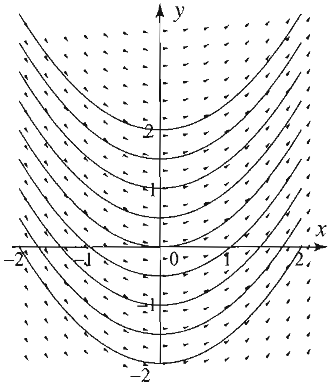
\includegraphics[height=4cm]{2_1.png}

O zaman PDE'nin genel cozumu 

\[ u(x,y) = f(C) = f(y - \frac{1}{2}x^2) \]

diyebiliriz, $f$ rasgele bir fonksiyondur, soylenmeye ugrasilan farkli
sabitlere tekabul eden $u$'lardir. PDE cozumu $u$'nun sabite esit olmasiyla
alakali cunku PDE'yi yonsel turev olarak temsil edince bu sonuca
variyoruz. Ustteki denklem de karakteristik egriler acisindan gelerek o
sabiti bize sagliyor.

$f$'in genel cozum oldugunu ana denklemde yerine koyarak test edebiliriz.

Ornek 

\[ u_x + yu_y = 0 \]

O zaman 

\[ \frac{dy}{dx} = y \]

\[ y = Ce^x \]

ya da

\[  C = e^{-x}y\]

Genel cozum 

\[ u(x,y) = f(C) = f(e^{-x}y) \]

PDE icinde yerine koyarak sonucu kontrol edelim

\[ u_x + yu_y = 
-f'(e^{-x}y)e^{-x}y + y f'(e^{-x}y) e^{-x} = 0
 \]

* * *

Dalga Denklemi 

\[ u_{tt} = c^2 u_{xx} \]

dalga denklemi olarak bilinir. Bir diger sekilde 

\[ u_{tt} - c^2 u_{xx} = 0\]

Bu denklemi operatorlerin faktorize edilmis hali olarak gormek mumkundur. 

\[ u_{tt} - c^2 u_{xx} = 
\bigg( \frac{\partial }{\partial t} - c \frac{\partial }{\partial x} \bigg)
\bigg( \frac{\partial }{\partial t} + c \frac{\partial }{\partial x} \bigg)
u = 0
\ \ \ (3)
\]

Esitligin sag tarafindaki operatorler hakikaten dalga denklemine tekabul
ediyor mu? Kontrol edelim, ustteki $u$ uzerinde etki eden ilk operator su
sekilde aciliyor

\[ \bigg( \frac{\partial }{\partial t} + c \frac{\partial }{\partial x}
\bigg) u = 
\frac{\partial u}{\partial t} + c \frac{\partial u}{\partial x}
\]

Simdi ikinci operatoru uygulayalim (bu sefer eksi olan operator), yani sunu
hesaplayalim, ve ustteki esitligin sag tarafi soyle olur

\[ 
\bigg( \frac{\partial }{\partial t} - c \frac{\partial }{\partial x} \bigg)
\frac{\partial u}{\partial t} + c \frac{\partial u}{\partial x} 
 \]

\[ = 
\frac{\partial ^2 u}{\partial t^2} + 
c \frac{\partial u}{\partial x \partial t} - 
c \frac{\partial u}{\partial t \partial x} - 
c^2\frac{\partial ^2 u}{\partial x^2} 
 \]

$u_{xt} = u_{tx}$ olduguna gore ortadaki iki terim iptal olur

\[ = 
\frac{\partial ^2 u}{\partial t^2} -
c^2\frac{\partial ^2 u}{\partial x^2} 
 \]

Acilimi ispatlamis olduk. 

Cozumu bulalim. Karakteristik kordinat (characteristic coordinate)
yontemini kullanalim. Bu sefer ilginc bir sey yapacagiz, kordinat
degisimini tanimlayan esitliklerden sonra operatorler uzerinde sanki
cebirsel buyukluklermis gibi islem yapacagiz. 

\[ \xi = x + ct \]

\[ \eta = x - ct \]

Bu kordinat degisimi icin bir tahmin yuruttuk. Dogru olup olmadigini simdi
gorecegiz. 

\[ \partial_x = \partial_\xi + \partial_\eta \]

\[ \partial_t = c\partial_\xi - c \partial_\eta \]

Bu formuller aslinda 1. derste gordugumuz (1),(2) formullerine benziyor,
sadece usttekiler pur operator formunda ve sabitler bu probleme gore
ayarli. 

Simdi iki ustteki formulu $c$ ile carpip bir ustteki formul ile toplarsak,
sonuc 

\[ \partial_t + c\partial_x = 2c \partial_\xi \]

Toplamak yerine bir ustteki formulden iki ustteki formulu cikartirsak

\[ \partial_t - c\partial_x = -2c \partial_\eta \]

Ustteki esitliklerin sol taraflari, daha once PDE icin operator acilimi
yaptigimizda ortaya cikan operatorler ile ayni. O zaman acilimda yerlerine
koyarsak, PDE soyle olur

\[ (2c\partial_\xi)(-2c\partial_\eta)u = 0 \]

Diger bir deyisle 

\[ u_{\xi_\eta} = 0 \]

Biliyoruz ki $c \ne 0$. Bu transform edilmis denklemin cozumu nedir? Ilk
once $\eta$'ya gore entegral aliriz, 

\[ u_\xi = f(\xi) \]

Bir daha entegral aliriz

\[ u = F(\xi) + G(\eta) \]

ki $F' = f$ olarak alindi. Burada aslinda $f,F$'in ne olduklari pek onemli
degil, ikisi de rasgele fonksiyonlar, tek onemli olan aldiklari
parametreler. O zaman cozum 

\[ u(x,t) = F(x+ct) + G(x-ct) \]

ki $F,G$ rasgele fonksiyonlar. 


\end{document}
